\chapter{Anforderungsanalyse}
Erreger in Krankenhäusern spielen eine immer größere Rolle, da mittlerweile Multiresistente Keime in Krankenhäusern existieren \cite{Niknam2017} und Menschen mit hoch ansteckenden Krankheiten behandelt werden. Nach jeder Operation und jedem chirurgischen Eingriff sind medizinische Instrumente potentiell mit Keimen kontaminiert. Die Sterilisation, also die Entfernung von Keimen jeder Art ist Aufgabe der Zentralen Serilgutversorgung. \todo{...}
%
% - - - - - - - - - - - - - - - - - - - - - - - - 
%
\section{Ablauf der Medizinprodukteaufbereitung}
% 2 Seiten
Sterile chirurgische Instrumente werden in verschiedenen Abteilungen von Krankenhäusern und Kliniken verwendet. Sterile Instrumente werden in sterilen Verpackungen und -Containern transportiert und bis zu ihrem Einsatz steril gehalten. Bei ihrem Einsatz werden die Instrumente verschmutzt und potentiell kontaminiert. Sie werden anschließend gesammelt und zur ZSVA geliefert \cite[S.~7]{Ruther2014}.

Kontaminierte chirurgische Instrumente werden zum unreinen Bereich der ZSVA transportiert. Die Instrumente werden häufig mit Zusatzinformationen zu ihrem Zustand geliefert. Ein Angestellter der ZSVA ordnet die Instrumente nach Kategorien in Container ein. Die Zuordnung geschieht mittels Barcodes, die an den Instrumenten befestigt sind \cite[S.~9]{Ruther2014}.

Im anschließenden Reinigungsverfahren werden die Instrumente aus ihren Containern entfernt und meist in Reinigungsmaschinen gegeben. Manche Instrumente müssen jedoch von Hand gereinigt werden. Bei der Reinigung soll der Kontakt zwischen Mitarbeiter und Sterilgut so gering wie möglich gehalten werden. 

Nach der Reinigung wird das Sterilgut desinfiziert. Zu einer sichereren Desinfektion müssen die Geräte korrekt in Gitter einsortiert werden. Dabei hat jedes Instrument spezifische Eigenschaften, die beachtet werden müssen \cite[S.~11]{Ruther2014}.

Nachdem das Sterilgut desinfiziert wurde, wird es in den Sterilbereich der ZSVA überführt. Von nun an gilt es als Steril. Hier werden die Instrumente nochmals auf äußere Einflüsse hin untersucht. Spezielle Wünsche des Kunden, wie der Ersatz bestimmter Komponenten wird nun berücksichtigt. Es werden anschließend Beschriftungen an den Sterilgütern befestigt, die mittels eines Barcode-Lesers ausgelesen werden können.
Die Beschriftungen enthalten neben dem Barcode den Namen des Instruments oder Container und das Ablaufdatum, an dem die Sterilität abläuft. Das Sterilgut wird anschließend so verpackt, dass die Instrumente und Container bis zu ihrem Einsatz steril bleiben. Für jedes chirurgische Instrument gibt es eine charakteristische Anleitung, wie das Sterilgut zu verpacken ist.

\begin{figure}[htbp]
    \centering
    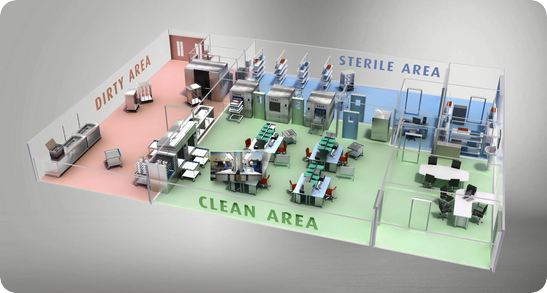
\includegraphics[width=1\textwidth]{data/bilder/clean-area-sterile-area.png}
    \caption{Schematischer Aufbau der Sterilgutversorgung \cite{Ives2017}}
    \label{fig:AufbauDerSterilgutversorgung}
\end{figure}

Wie in Abbildung \ref{fig:AufbauDerSterilgutversorgung} schematisch gezeigt, besteht die ZSVA aus drei Abschnitten: einer kontaminierten und unsauberen, einer sauberen und einer sterilen Abteilung. Diese drei Bereiche sind durch Desinfektions- und Sterilisationsmaschinen getrennt. Diese bilden eine Hygiene-Barriere zwischen den verschiedenen Hygieneleveln. Zwischen den unreinen- und reinen Bereichen bestehen Durchreichen, um Instrumente zwischen den Bereichen zurückreichen zu können, falls diese nicht korrekt gereinigt und desinfiziert wurden. \cite[S.~24]{Ruther2014}. Sterilgut kann nach der Behandlung in den Maschinen sehr heiß sein, was dazu führt, dass Mitarbeiter der Sterilgutversorgung strenge Sicherheitsvorkehrungen einhalten müssen sowie spezielle Kleidung tragen müssen. Dies ist besonders in der unreinen Abteilung nötig, da ebenfalls verhindert werden muss, dass sich Mitarbeiter mit Infektionen anstecken. Medizinische Instrumente sind mit Barcodes ausgestattet, welche in verschiedenen Schritten des Arbeitsprozesses ausgelesen werden. Computer sind essentieller Bestandteil der ZSVA, insbesondere der Reinabteilung. Hier unterstützen Softwarelösungen Mitarbeiter bei der Zusammenstellung der Instrumente. \cite[S.~25]{Ruther2014}.
%
% - - - - - - - - - - - - - - - - - - - - - - - - 
%
\section{Anforderungen bei der Medizinprodukteaufbereitung}
% 3 Seiten
In der Medizinprodukteaufbereitung werden mehrere tausend verschiedene medizinische Instrumente aufbereitet. Diese können sehr einfach bis sehr komplex strukturiert sein. Angestellte stehen oft unter hohem Zeitdruck und sind vielen Sicherheits- Hygienebestimmungen ausgesetzt. Es gibt zudem viele Fehlerquellen bei der korrekten Durchführung von Anweisungen, da Angestellte nicht immer alle Anweisungen und Anleitungen zu allen verschiedenen Instrumenten und allen einzelnen Prozesschritten kennen können.

In den heutigen ZSVAs finden sich typischerweise Barcodescanner für die automatische Prozessdokumentation. Instrumente werden in einem Behälter mit einem eindeutigen Identifizierungsetikett (Barcode) gesammelt. Für jeden Prozessschritt wird der Barcode gescannt und der Prozessschritt automatisch dokumentiert.

Angestellte im unreinen Bereich könnten von einem Assistenzsystem profitieren. 
In diesem Umfeld, in dem Oberflächen verschmutzt und kontaminiert sind, müssen spezielle hygienische Anforderungen erfüllt werden. So muss Sicherheitskleidung getragen werden. Klassische Desktop-Computer sowie Touchscreens sind hier aus hygienischen Gründen nicht einsetzbar.  \cite[S.~28]{Ruther2014}. Ein Assistenzsystem muss zudem abwaschbar sein und steril gehalten werden können. Es muss also möglich sein, die Hardware im unreinen Bereich anzuwenden. 

Eine wichtige Anforderung an Assistenzsysteme ist zudem die Akzeptanz durch die Anwender. So spielt die Benutzerfreundlichkeit des Systems eine wichtige Rolle. Das System sollte den regulären Workflow der Angestellten weder verzögern noch stören. Informationen müssen präzise und Kontextabhängig angezeigt werden. So muss der Angestellte selbst entscheiden können, zu welchem Instrument Zusatzinformationen angezeigt werden, da viele Instrumente und deren Behandlung wohl bekannt sind. Für diese Instrumente werden keine Zusatzinformationen benötigt und das System sollte keine Rolle spielen. Für unbekanntere und komplexere Instrumente müssen jedoch schnell Informationen angezeigt werden können, damit der Arbeitnehmer unterstützt werden kann. \cite[S.~29]{Ruther2014} \todo{...}
%
% - - - - - - - - - - - - - - - - - - - - - - - - 
%
\section{Smartglasses im Bereich der Medizinprodukteaufbereitung}
\label{sec:Smartglasses_im_Bereich_der_Medizinprodukteaufbereitung}
Im Folgenden werden die Einsatzmöglichkeiten von Smartglasses beleuchtet. Anschließend werden die spezifischen Anforderungen an Smartglasses in diesem Einsatzbereich analysiert und abschließend Datenschutzrechtliche sowie Arbeitsschutzrechtliche Aspekte des Einsatzes von Smartglasses beleuchtet.
%
% - - - - - - - - - - - - - - - - - - - - - - - - 
%
\subsection{Einsatzmöglichkeiten}
\label{sec:Einsatzmoeglichkeiten}
% 4 Seiten
Heute müssen Angestellte der ZSVA zur Arbeit mit IT-Systemen an stationären Arbeitsplätzen arbeiten. Mobile Geräte wie Tablets erfordern eine Bedienung mit den Händen. Smartglasses dagegen sind immer einsatzbereit und ermöglichen völlig freihändiges Arbeiten. Sie ermöglichen den permanenten Zugriff auf Informationen und können so auch außerhalb des regulären Arbeitsplatzes eingesetzt werden. So können Angestellte der ZSVA auch beidhändig arbeiten. Beidhändiges Arbeiten ist in der ZSVA von großer Bedeutung.

Mithilfe der eingebauten Foto- und Videokamera können Arbeitsschritte lückenlos aufgezeichnet und dokumentiert werden. So können defekte oder problembehaftete Instrumente schnell dokumentiert werden.

Mithilfe von Smartglasses können Anleitungs- und Hilfevideos erstellt und abgerufen werden. So können erfahrene Angestellte für ihre unerfahreneren Kollegen Videos anfertigen, die zu einer Unternehmensinternen Wissensdatenbank erweitert werden können. Schritt-für-Schritt- Anleitungen können überforderungen von Mitarbeitern entgegenwirken und so die Arbeitsqualität erhöhen.

Schritt-für-Schritt Anleitungen erhöhen zudem die Flexibilität von Mitarbeitern im Unternehmen, da diese so an verschiedenen Stellen der Medizinprodukteaufbereitung eingesetzt werden können und dank der Unterstützung der Datenbrille möglicherweise auf Schulungen verzichten können. Monotonen Tätigkeiten wird somit ebenfalls vorgebeugt, da Angestellte so in verschiedenen Bereichen der ZSVA eingesetzt werden.

Treten Probleme im Arbeitsalltag auf, können Smartglasses auch dazu genutzt werden, mithilfe der Videokamera mit anderen Kollegen zu kommunizieren. So kann einem Gesprächspartner per Video das betreffende Sterilgut gezeigt werden und so schnell eine Lösung gefunden werden.

Smartglasses können auch dazu eingesetzt werden, Angestellte vor Gefahren zu warnen. So können Fehler im Arbeitsalltag verhindert werden und Prozesse sicherer gestaltet werden.

Smartglasses bieten nicht nur den immer perfekt eingestellten Bildschirm, der unabhängig von der Körpergröße des Anwenders ist, sondern lassen sich auch individualisieren. So kann ein Mitarbeiter die Datenbrille nach seinem Kenntnisstand einstellen und individuell anpassen. So kann auf Qualifikation, Erfahrung und Computer-Affinität eingegangen werden.

Ein Lagersystem kann die Handlungen der Benutzer koordinieren und somit Nutzern mitteilen, in welchem Arbeitsschritt sich andere Mitarbeiter befinden. So können redundante Arbeitsschritte verhindert werden. 
\todo{...}
%
% - - - - - - - - - - - - - - - - - - - - - - - - 
%
\subsection{Spezifische Anforderungen an Smartglasses im Bereich der Medizinprodukteaufbereitung}
% 3 Seiten
Smartglasses im Bereich der Medizinprodukteaufbereitung müssen viele spezielle Anforderungen erfüllen. Es müssen im Gegensatz zu klassischen Computern mit Maus und Tastatur bzw. Touch-gesteuerten Geräten wir Tablets neuartige Bedienkonzepte verwendet werden. So lassen sich Smartglasses mittels Sparch- und Gestensteuerung bedienen.
Sprachsteuerung in der Medizinprodukteaufbereitung muss sehr sensitiv sein. In den Räumen, in denen die Brillen eingesetzt werden sollen herrscht ein sehr großer Hintergrundgeräuschpegel, welcher die Sprachsteuerung bei fehlender Noice-Cancellation massiv beeinträchtigen würde. Denkbar ist ebenfalls der Einsatz einer personenabhängigen Spracherkennung, da im Raum möglicherweise mehrere Nutzer Smartglasses mittels Sprachsteuerung bedienen bzw. normale Gespräche missinterpretiert werden könnten. 

Es ist nötig, neuartige User-Interfacesysteme zu entwickeln, die es ermöglichen, alle nötigen Informationen auf einem kleinen Display wie dem einer Datenbrille darzustellen. 

Smartglasses, die von Angestellten der ZSVA verwendet werden, müssen abwaschbar und steril gehalten werden können. Nur so kann es möglich sein, diese einzusetzen. Sie müssen also wasserdicht sein, ein einfacher Spritzwasserschutz reicht nicht aus. Zudem müssen die Brillen robust genug sein, um die aggressiven Reinigungs- und Desinfektionsmittel zu überstehen.

Smartglasses müssen aufgrund des ganztägigen Einsatzes zudem weitere Harwareanforderungen erfüllen. Sie müssen möglichst leicht sein, damit sie die Angestellten in ihrer Arbeit nicht beeinträchtigen. Der Bedienkomfort der Brille hat hier einen großen Stellenwert. 

Die Brille muss über einen ausreichend starken Akku verfügen, um mindestens einen 8 Stunden Arbeitstag durchzuhalten bzw. müssen einen austauschbaren Akku haben. Ebenfalls denkbar ist eine externe Stromquelle, die mittels eines Stromkabels an die Brille angeschlossen ist.

Aufgrund der großen Lautstärke im Bereich der ZSVA muss die Sprachsteuerung in der Lage sein, auch bei großen Hintergrundgeräuschen die Sprachsteuerung gewährleisten zu können. Ebenfalls sollte die Sprachsteuerung auf eine Person abgestimmt werden können, damit mehrere parallel sprechende Menschen sich nicht gegenseitig beeinträchtigen.

Anwendungen für Smartglasses in der Medizinprodukteaufbereitung benötigen eine ständige Verbindung ins Internet, um auf Datenbanken und externe Videos sowie Bilder zugreifen zu können. Falls ebenfalls eine Video-Streaming oder Videotelefoniefunktionalität implementiert werden soll, ist eine Unterstützung moderner und schneller Datenverbindungen realisiert sein. Da eine Mobilfunkverbindung in Gebäuden nicht garantiert werden kann und für größere Datenmengen nicht praktikabel ist, sollte die Brille über WLAN verfügen uns sich eigenständig ins Internet einwählen können ohne ein externes Smartphone zu benötigen.

Zur Identifikation von möglicherweise sehr kleinen Barcodes und QR-Codes sowie potentiell auch Gegenständen ist eine möglichst hochauflösende Kamera nötig. Diese sollte möglichst das Sichtfeld des Anwenders direkt erfassen können. Weitere Sensoren zur Bestimmung von anderen Medien, wie beispielsweise RFID-Codes, sind ebenfalls denkbar.\todo{...}

Nach Analyse der Anforderungen und Betrachtung der in Kapitel \ref{sec:VergleichSmartglasses} beschriebenen Smartglasses kommt die \emph{Realwear hmt-1} am ehesten in Frage. Sie ist abwischbar (Wasserfest), ist Robust genug und verfügt über einen lange anhaltenden Akku. Die Spracherkennung ist mittels einer aktiven Noice-Cancellation auch in lauter Umgebung wie der Medizinprodukteaufbereitung möglich. Sie verfügt über WLAN und ist auch ohne ein gekoppeltes externes Smartphone internetfähig. Die Kamera der Brille ist hochauflösend Genug, um auch kleine Barcodes und QR-Codes erfassen zu können.
%
% - - - - - - - - - - - - - - - - - - - - - - - - 
%
\subsection{Datenschutz}
Der Einsatz von Smartglasses wird in der Literatur in Datenschutzrechtlicher Hinsicht diskutiert \cite{Berkemeier2017}. Smartglasses stellen eine nicht zu ignorierende Einschränkung in das Grundrecht auf informationelle Selbstbestimmung dar und erfordern damit völlig neue Anforderungen des Datenschutzrechts.

Besonderheit beim Einsatz von Smartglasses ist, dass diese im Betrieblichen Einsatz durchgängig genutzt werden und somit nicht nur die Nutzer der Brille, sondern auch alle in ihrem Umfeld befindlichen Personen durch die Grundrechtseingriffe der Brille betroffen sind. Aus Sicht des Datenschutzes sind Smartglasses den invasiven Technologien und Werkzeugen zu zuordnen \cite{Berkemeier2017}. Somit muss der Datenschutzaspekt essenzieller Bestandteil beim Design informationstechnischer Systeme in Smartglasses sein. 

Der rechtliche Rahmen für den Einsatz von Smartglasses in Unternehmen wird derzeit vom Bundesdatenschutzgesetz (BDSG), jedoch zunehmend auch durch den europäischen Rechtsrahmen gesetzt. Die im Mai 2017 in Kraft getretene EU- Datenschutzgrundverordnung (DSGVO) bildet den allgemeinen Rahmen der Datenschutzleitlinien. Grundsätzlicher Nenner der Rechtsgrundlagen ist, dass die Datensouveränität und Privatsphäre der Betroffenen vor Technologien geschützt wird. So müssen Vorkehrungen getroffen werden, die Erhebung, Speicherung und Nutzung von Daten zu reglementieren.
Die DSGVO regelt die rechtskonforme automatisierte Datenverarbeitung, genauer die Erhebung, Verarbeitung und Nutzung, von personenbezogenen Daten \cite{Berkemeier2017}. Die DGSVO stellt dabei einen ausführlichen  Pflichtenkatalog für die Verarbeitung personenbezogener Daten auf. Der Umfang hängt dabei von der Intensität des Eingriffs ab. Es sollten also nur Daten erhoben werden, die keiner der besonders geschützten Kategorien zuzuordnen sind und dies nur im Aussmaß, die keine dauerhafte Speicherung erfordert. Werden personenbezogene Daten durch ein Unternehmen gespeichert, so setzt dies immer eine explizite Einwilligung voraus, die zu dokumentieren ist.

Smartglasses nehmen potentiell dauerhaft Video- und Tonaufnahmen auf und machen es möglich per Gesichtserkennung Personen im Umfeld des Nutzers zu identifizieren. \cite[S.~38f]{Schwenke2016} Es ist ebenfalls potentiell möglich, den Nutzer der Brille in seinem Handeln und Verhalten zu überwachen. Es muss also sichergestellt werden, dass diese personenbezogenen Daten nicht gespeichert werden \cite[S.~34]{Schwenke2016}. Die Brillen verfügen potentiell über eine Stimmerkennung, welche ebenfalls Muster über den Anwender ermöglicht \cite[S.~41]{Schwenke2016}. Diese Daten müssen zur Verwendung der Brille zwar gespeichert sein, sollten jedoch nicht auslesbar und verschlüsselt in der Smartglass gespeichert werden.

Die starke Bedeutung von Datenschutz in Verbindung mit Smartglasses zeigt sich auch in der Reaktion der Öffentlichkeit auf die Veröffentlichung von Google Glass im Jahr 2014. So wurde schnell der Begriff des \enquote{Glassholes} \cite[S.~14]{ThomasDirkMetzgerHelmutNiegemannHrsg2018} gebildet. Gemeint ist damit in abwertender Weise eine Person, die durch eine Google Glass eine permanent potentiell aufnehmenden Kamera auf Mitmenschen richtet. Für den beruflichen Kontext kann diese Problematik dann Anwendung finden, wenn Personen aufgezeichnet werden, die kein Einverständis gegeben haben. Bei der Veröffentlichung von Google Glass wurde die Erfindung zwar einerseits vom Time-Magazine als eine der \enquote{Best Inventions of the Year} gekürt \cite{Bilton2015}, jedoch kamen sofort auch kritische Stimmen auf, die die Gefahr für die Privatsphöre aufzeigten. So wurde der Zugang zu öffentlichen Einrichtungen wie Kinos oder Kasinos, mit einer Google Glass eingeschränkt \cite[S.~67]{Schwenke2016}. 

Smartglasses im beruflichen  sowie im privaten Kontext schränken bei einer fehlenden Zustimmung des betroffenen die Persönlichkeitsrechte der Nutzer und deren Umgebung ein. So schränken Smartglasses das Recht auf informationelle Selbstbestimmung ein \cite[S.~100]{Schwenke2016}, da sie bei fehlendem Einverständnis einen Kontrollverlust über personenbezogene Daten mit sich zieht. Wird ein Nutzer bei der Benutzung überwacht und werden diese bei der Nutzung generierten Daten gespeichert, so verliert der Nutzer die Hoheit über seine personenbezogene Daten. Werden beispielsweise durch die Brille Personen in Bild oder Video aufgezeichnet, diese Bilder gespeichert oder weitergegeben, so kommt es zu einem Konflikt, da der Nutzer das Recht am eigenen Bild hat \cite[S.~104ff]{Schwenke2016} \cite[S.~109f]{Schwenke2016}. 
Ein ähnlicher Konflikt liegt vor, wenn Gegenstände gefilmt werden, da so auch das Recht auf informationelle Selbstbestimmung verletzt werden kann, wenn beispielsweise Gegenstände gefilmt werden, die einen direkten Bezug zu Personen haben (Nummernschilder, Namensschilder, etc.) \cite[S.~106]{Schwenke2016}. 

Ein weiterer wichtiger Aspekt, die beachtet werden muss ist der Umgang mit personenbezogenen Daten. Der zu schützende Datenumfang umfasst dabei jede Form der
\enquote{Erhebung, schlichter Kenntnisnahme, Speicherung, Verwendung, Weitergabe oder Veröffentlichung von persönlichen – d.h. individualisierten oder individualisierbaren – Informationen} \cite[S.~108]{Schwenke2016}.

Werden Tonaufnahmen von Personen gemacht, so wird möglicherweise das Recht am nicht öffentlich gesprochenen Wort verletzt. Dieses garantiert jeder Person die \enquote{Garantie einer ungestörten zwischenmenschlichen Kommunikation} \cite[S.~112]{Schwenke2016}.

Smartglasses beschränken möglicherweise auch das Recht der Selbstbewahrung, also das Recht auf Privatsphäre. Dies kann auch im beruflichen Kontext eine Rolle spielen, wenn Angestellte beispielsweise in ihren Pausen gefilmt werden \cite[S.~114f]{Schwenke2016}.

Verwenden Smartglass-Apps biometrische Erkennungsverfahren wie Gesichtserkennung, wo Personen anhand ihrer physiologischen Charakteristika, d.h. der Gesichtsform und den Gesichtszügen identifiziert werden, so werden ebenfalls Persönlichkeitsrechte verletzt. Ebenso verhält es sich, wenn durch die Nutzung der Brille Verhaltenserkennung stattfinden kann und so eventuell Profile der Angestellten erstellt werden können.

Die Speicherung der Daten erfordert ebenfalls genauere Betrachtung: Speicherort, Speicherdauer, Übermittlung und Zugriffsmöglichkeiten Dritter auf Daten müssen beachtet werden. Werden die Daten auf der Brille selbst gespeichert, so bringt dies eine geringe Beeinträchtigung mit sich, solange keine Dritten Zugriff auf die Daten haben. Werden die Daten allerdings auf einem Server (\emph{Cloud-Dienste}) gespeichert, so müssen die jeweiligen Datenschutzbestimmungen beachtet werden. Hier ist auch die gesetzliche Regelung zur Speicherdauer und der Regelungen zur sicheren (verschlüsselten) Übermittlung der Daten zu beachten \cite[S.~165f]{Schwenke2016}.

Es kann also zusammenfassend davon ausgegangen werden, dass bei einer nicht- Zustimmung betroffener Personen, Persönlichkeitsrechte bei Bild- oder Tonaufnahmen sowie der Verwendung der Brille verletzt werden können. Erleichtert werden kann dieser Eingriff, wenn die Datenbrille beispielsweise wie bei der \emph{Epson Moverio BT-200} (vgl. Abschnitt \ref{sec:Epson_Moverio_BT-200}) über eine kleine Leuchtdiode verfügt, die die Kameranutzung bzw. deren Aufnahme impliziert \cite[S.~161]{Schwenke2016}. All diese möglichen Verletzungen der Persönlichkeitsrechte lassen sich mit einer Einwilligung der betroffenen Personen lösen, was im beruflichen Umfeld - vor allem in einem geschlossenen System wie der Medizinprodukteaufbereitung - möglich ist. So werden umfassende schriftliche Einwilligungen aller betroffenen Personen, also sowohl der Nutzer der Brille als auch aller Personen im Umfeld der Benutzer der Brille, benötigt \cite[S.~139f]{Schwenke2016}.
%
% - - - - - - - - - - - - - - - - - - - - - - - - 
%
\subsection{Arbeitssicherheit}
% 0,5 Seiten
Arbeitssicherheit spielt besonders in einem hoch infektiösen Umfeld wie der Medizinprodukteaufbereitung eine große Rolle.

Angestellte der Medizinprodukteaufbereitung müssen in ihrer Arbeit hoch konzentriert sein, da sie in der Gefahrenlage arbeiten, sich bei einem Fehler mit hochinfektiösen Bakterien oder Viren anzustecken. So darf eine eingesetzte Smartglass diese Aufmerksamkeit nicht beeinträchtigen. Da Smartglasses unterschiedlich gebaut sind, müssen diese auch getrennt betrachtet werden. Smartglasses im Stile von \emph{Google Glass} haben ein transparentes Display, welches im Sichtfeld des Betrachters liegt. Es ist möglich, durch den Bildschirm zu schauen und nur nach Bedarf Informationen im Rahmen der assistierten Realität anzuzeigen. Andere Smartglasses wie die \emph{Realwear hmt1} haben ein nicht- transparentes Display und schränken das Sichtfeld des Nutzers deutlich mehr ein. Hier kann es schneller zu einer Ablenkung seitens der Brille kommen. Ebenfalls wichtig ist, dass die Brille nur assistierend zur Seite stehen darf und nur bei Bedarf hinzugezogen werden sollte.

In der ZSVA werden meist Schutzbrillen getragen. Eine Smartglass darf diese Schutzbrille nicht ersetzen, sondern nur ergänzend getragen werden.

Smartglasses haben bei manchen Menschen den Effekt der sogenannten \enquote{virtual sickness} oder auch \enquote{Virtual reality sickness} kommen. Dieser Effekt tritt ein, wenn zu viel auf den Bildschirm geschaut wird. Der Effekt tritt besonders bei VR-Brillen auf, kann jedoch auch bei AR-Smartglasses auftreten, wenn der Raum, in dem sich die Person befindet, durch die Smartglass verändert und Bewegung des Nutzers nicht mit der Bewegung in der virtuellen Realität bzw. der augmentierten Realität übereinstimmt \cite{Moss2011}. Treten diese Symptome bei einem Angestellten gehäuft auf, sollten Pausen eingelegt werden oder Aufgaben übernommen werden, in der keine Smartglass benötigt wird.

Smartglasses können aber auch sehr gut im Sinne der Arbeitssicherheit eingesetzt werden. So kann die Assistenz durch die Brillen Unfälle verhindern, da Nutzer geschult sind und ggf. bei unbekannten Tätigkeiten Informationen abrufen können. Dies schützt vor allem ungeschulte Angestellte davor, möglicherweise gesundheitsgefährdende Fehler zu machen. Die Möglichkeit Hilfe heranzuziehen schützt somit vor gefährlichen Unfällen.
%
% - - - - - - - - - - - - - - - - - - - - - - - - 
%
\subsection{Grenzen des Einsatzes von Smartglasses}
% 2 Seiten  
Der Einsatz von Smartglasses im Bereich der Augmented Reality ist beschränkt. Da es sich bei Smartglasses, wie in Kapitel \ref{sec:Einordnung_von_Smartglasses} gezeigt, um Brillen der assistierten Realität handelt, bieten diese nicht die vollen Möglichkeiten von \emph{echten} AR-Brillen. Es können nur kontextsensitive Informationen eingeblendet werden und mittels Interaktion verarbeitet werden. Wirkliche Augmented Reality- oder sogar Virtual Reality- Effekte sind hier jedoch garnicht erwünscht und benötigt.%
\todo{...}